\section*{Regression Visualization}

    \subsection*{Visualizing our Model}
    
        With \textbf{one variable}, we've seen that our linear model simply turns into $\theta_1 x_1  + \theta_0$. As you'd expect, on a plot, this looks like a \textbf{line} in the \textbf{2D plane}.
        
        \begin{figure}[H]
        \centering
            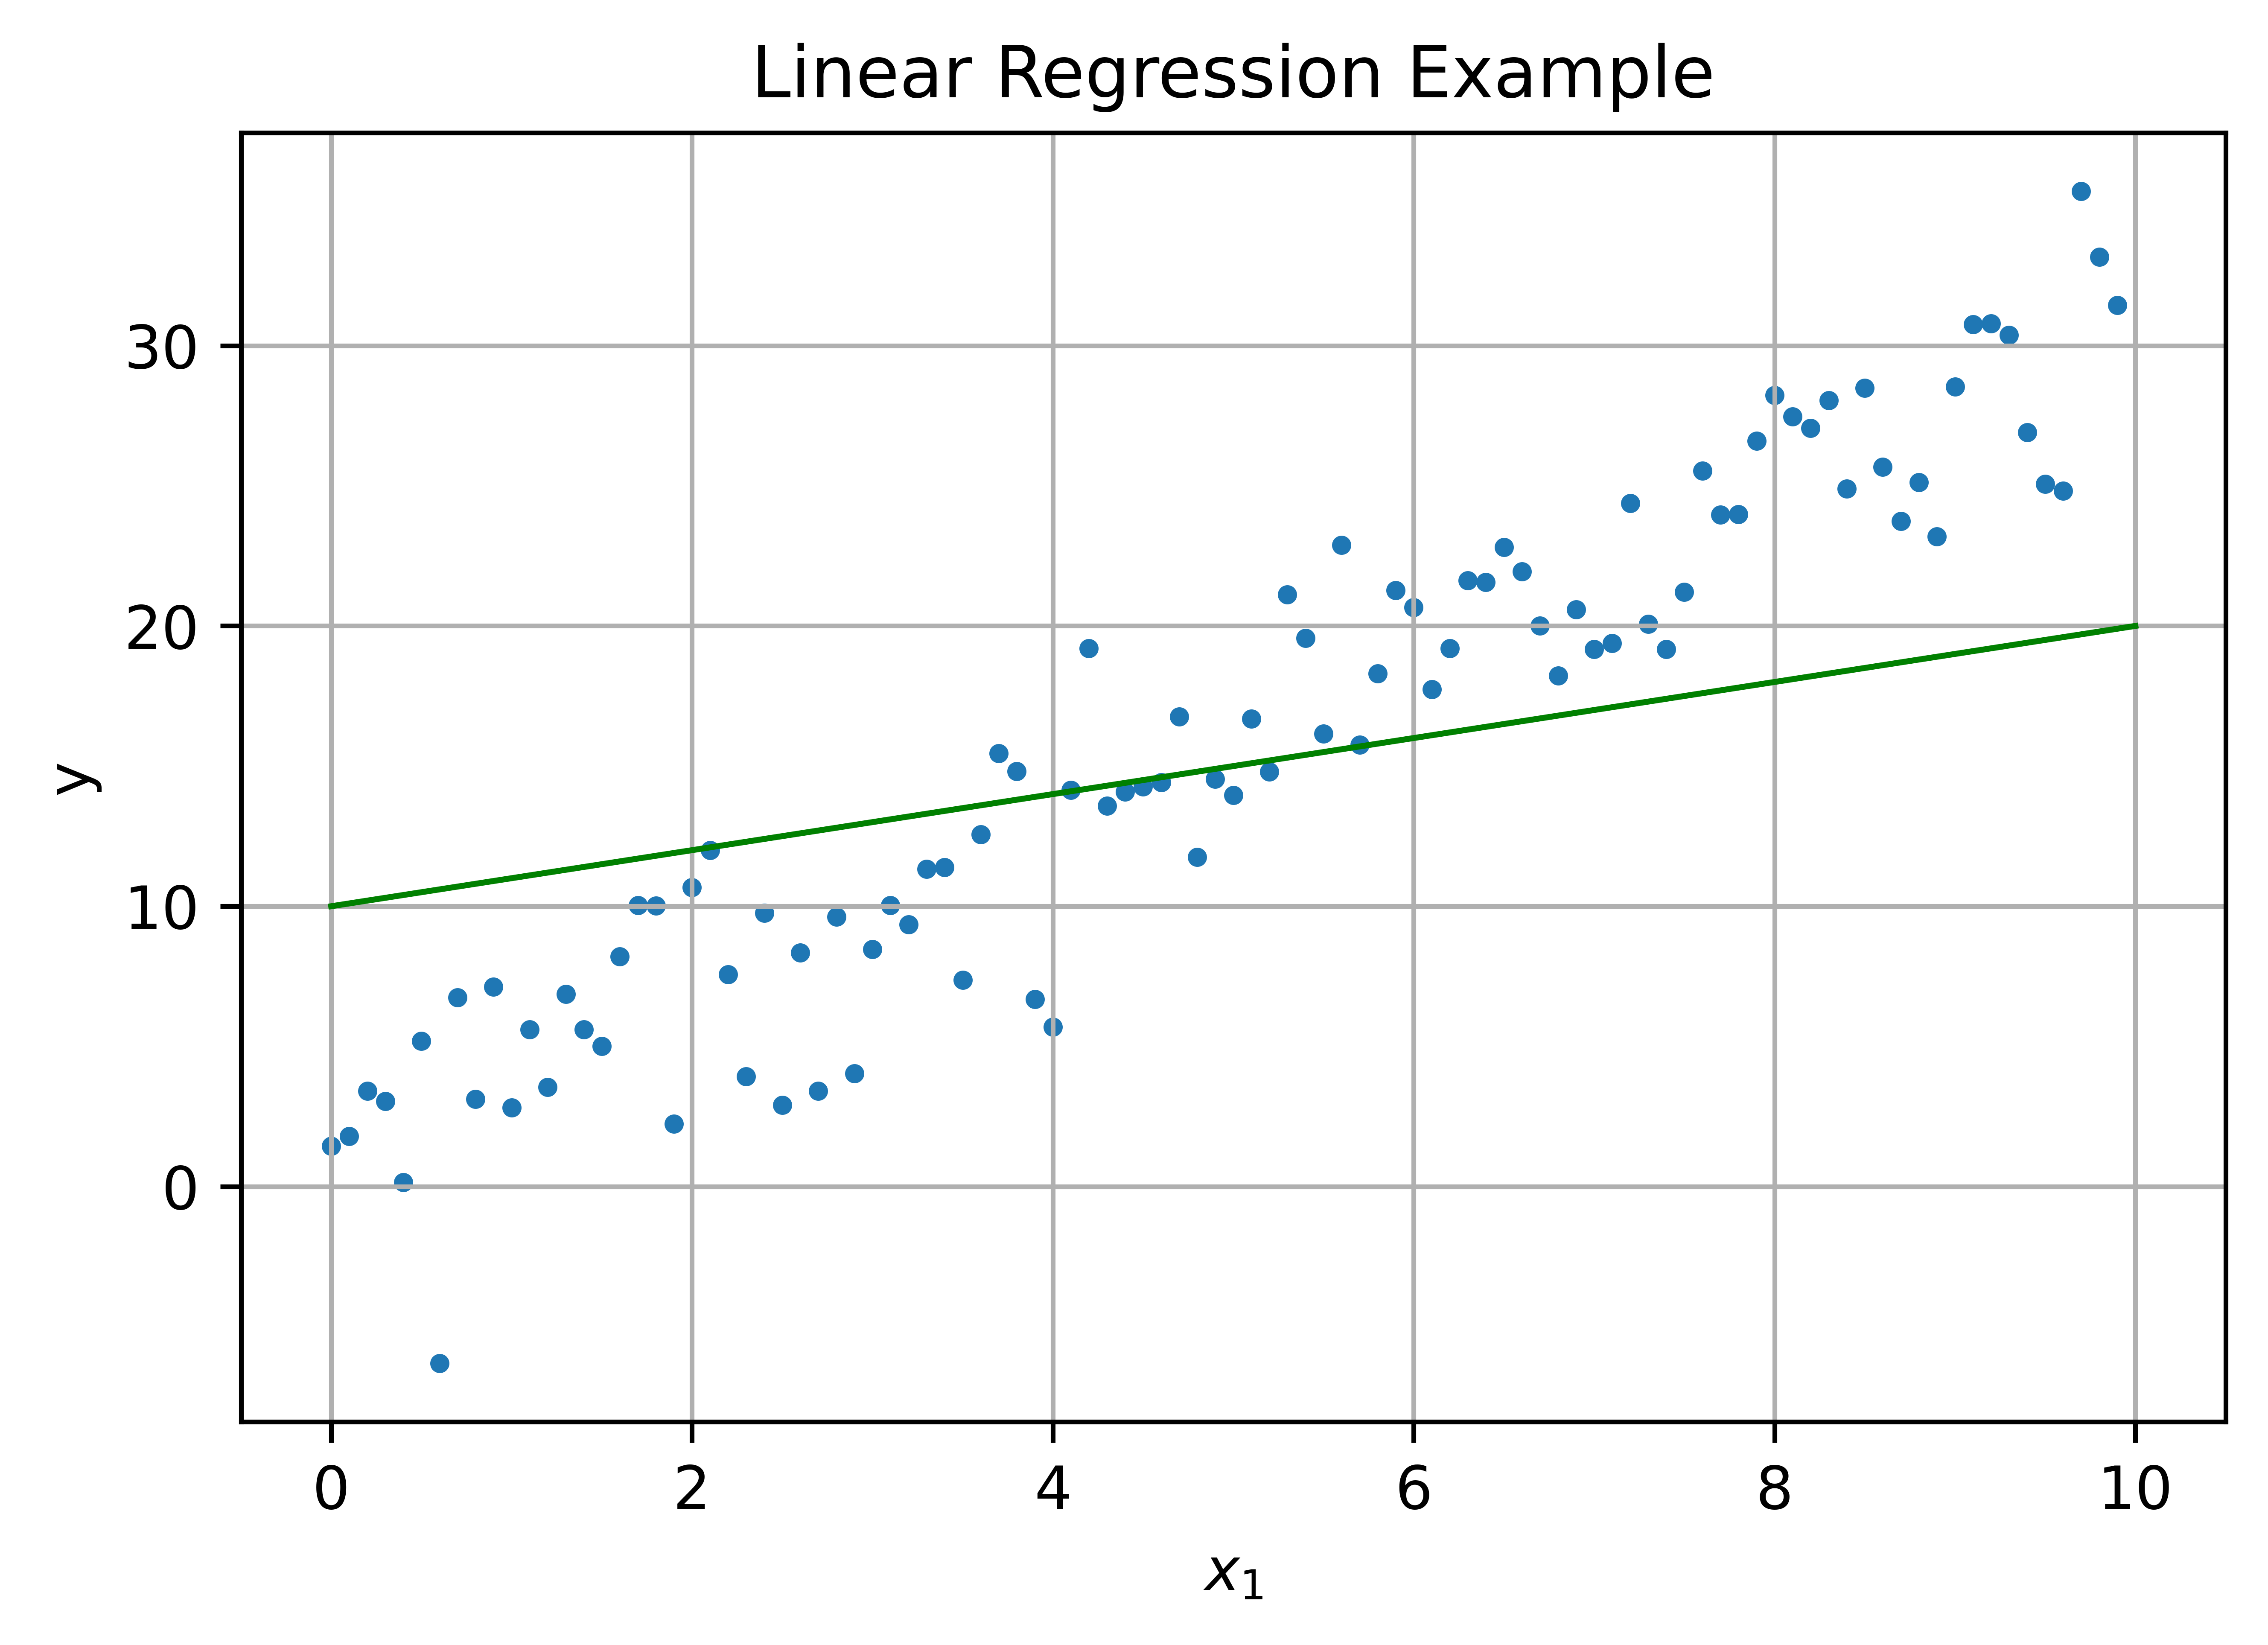
\includegraphics[width=70mm,scale=0.5]{images/regression_images/Regression_Example_Poor_Fit.png}
        
            \caption*{This example of linear regression is not a great fit: $(\theta_0=10, \theta_1=1)$}
        \end{figure}
        
        We're trying to get our line as \textbf{close as possible} to the points, hoping to find a linear pattern. We're \textbf{fitting} our line to the data.
        
        \begin{figure}[H]
        \centering
            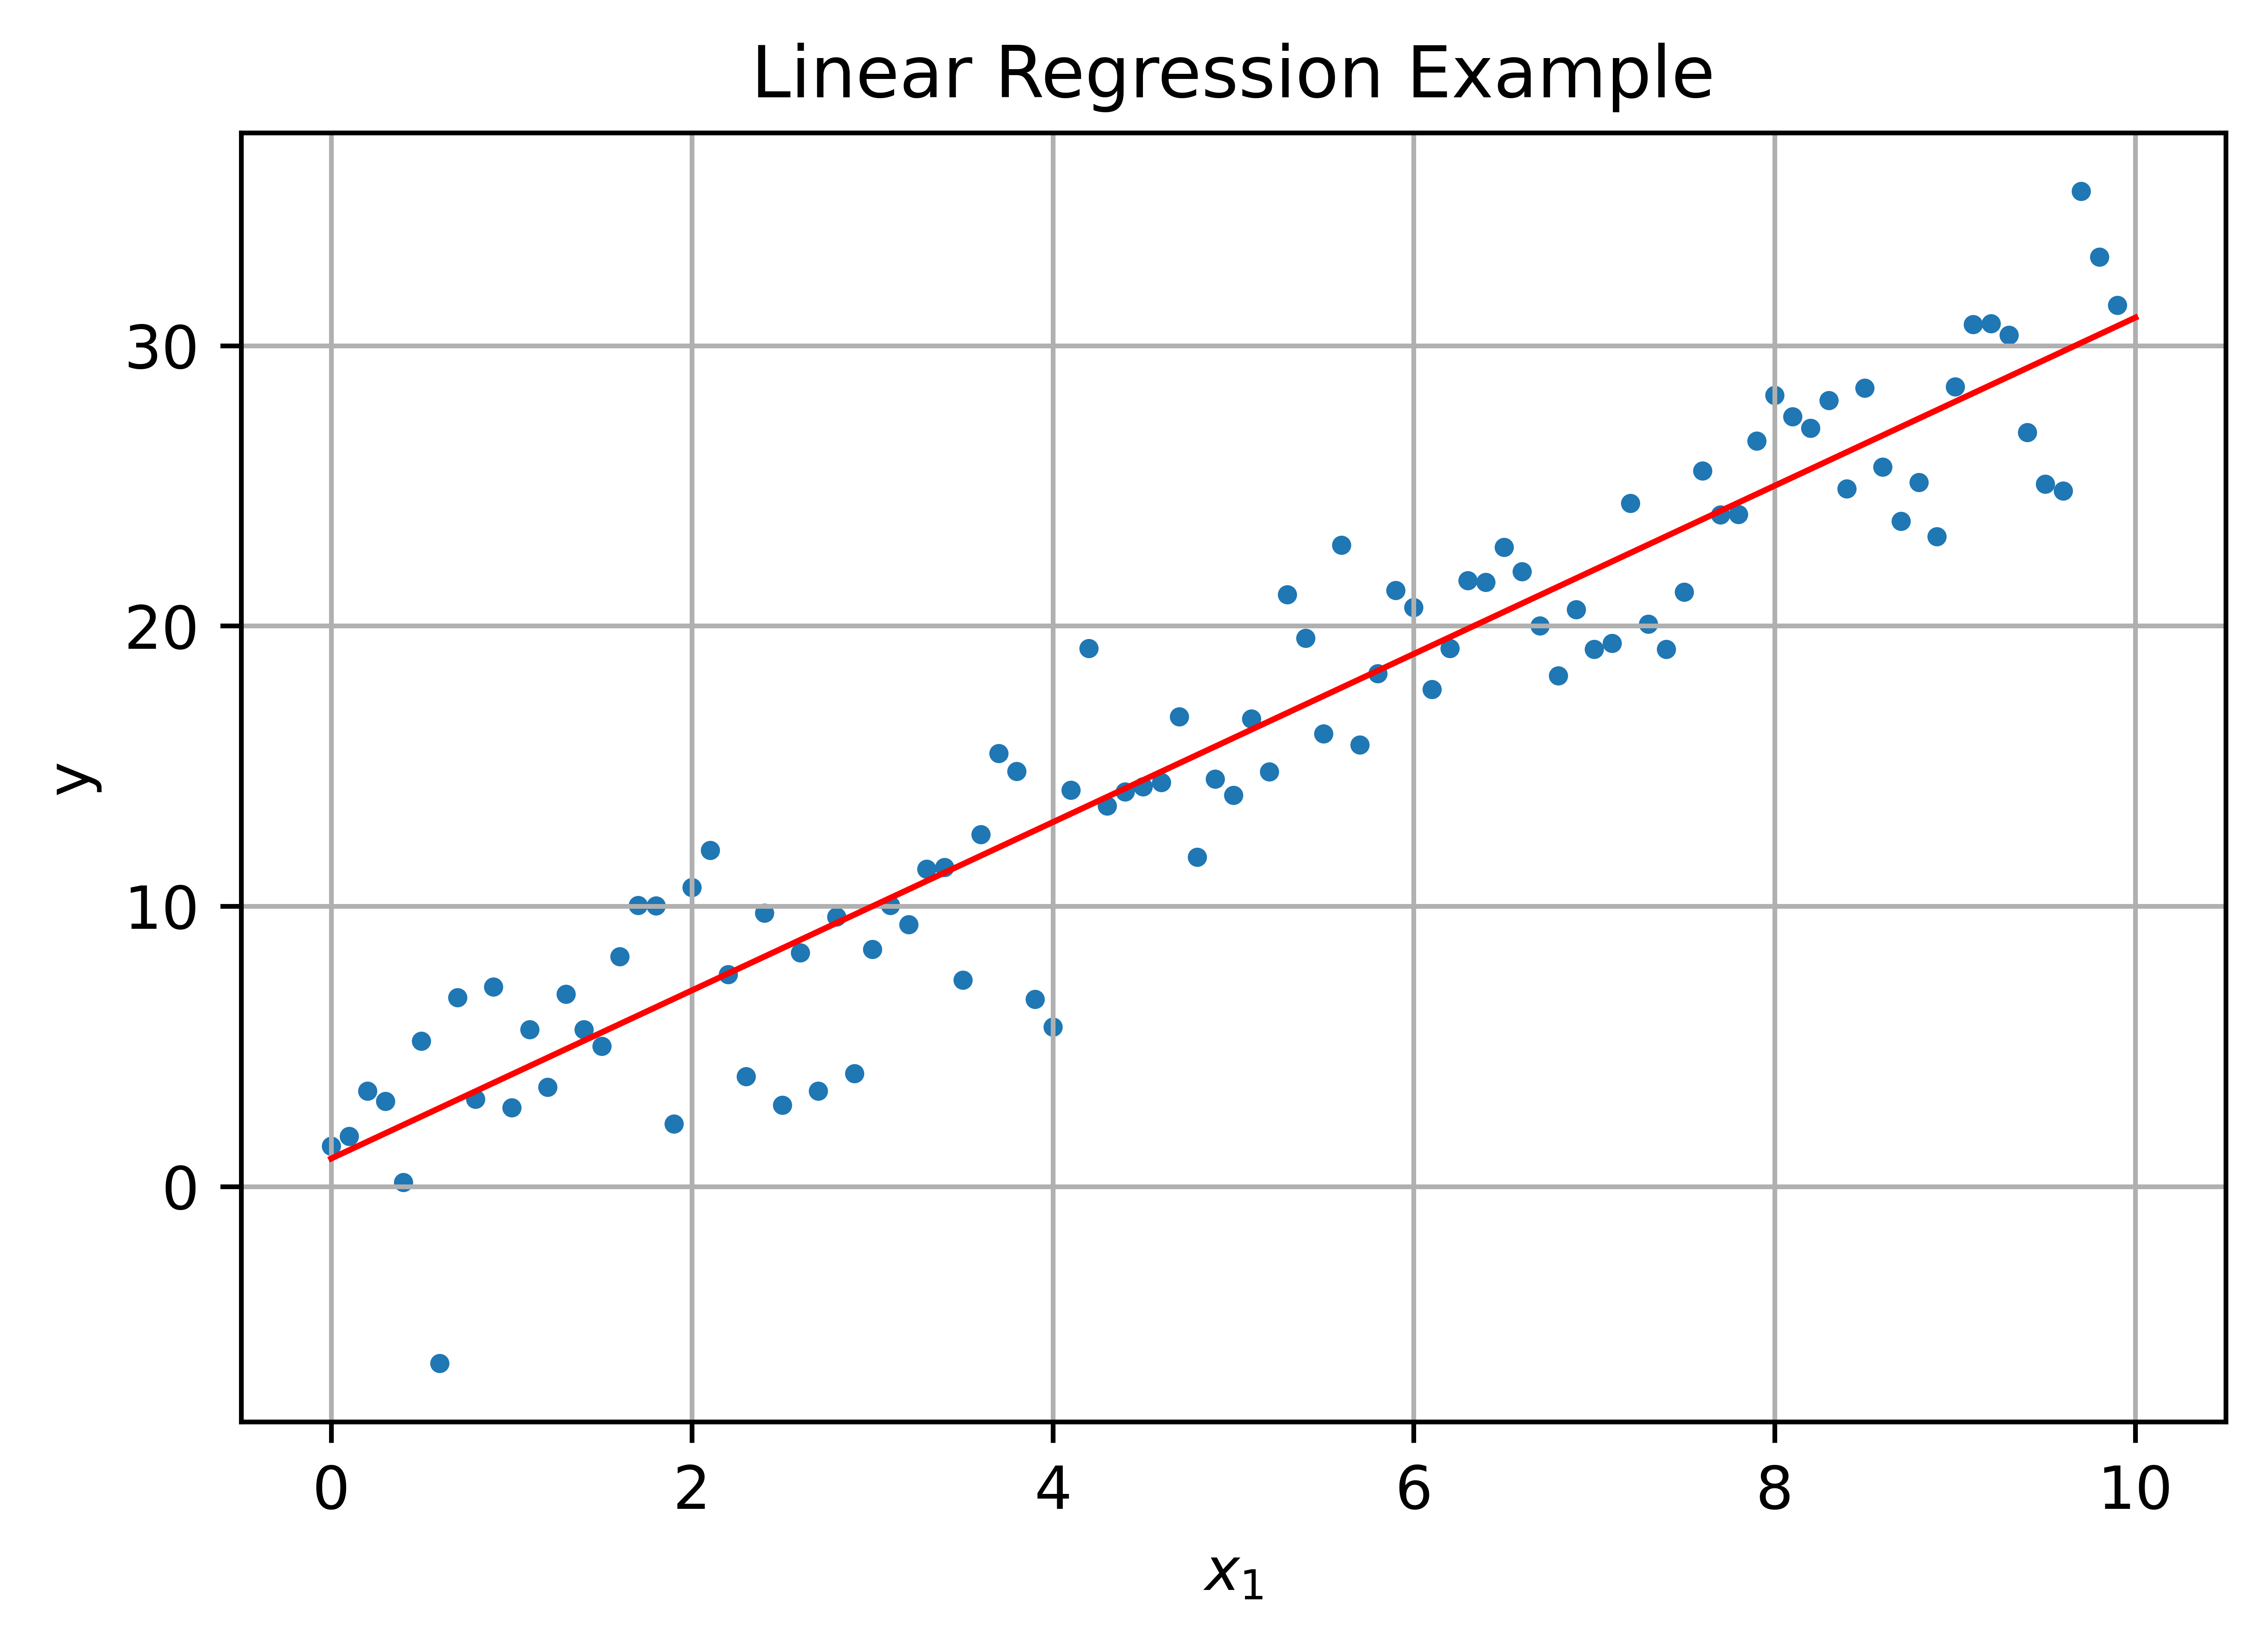
\includegraphics[width=70mm,scale=0.5]{images/regression_images/Regression_Example_Good_Fit.png}
        
            \caption*{This line is much better fitted to the data: $(\theta_0=1, \theta_1=3)$}
        \end{figure}
        
        What does this like if we have \textbf{two} variables? You need a 3D space, with 2 dimensions for the input.
        
        Extending our line into a second dimension, we create a \textbf{plane}.
        
        \begin{figure}[H]
        \centering
            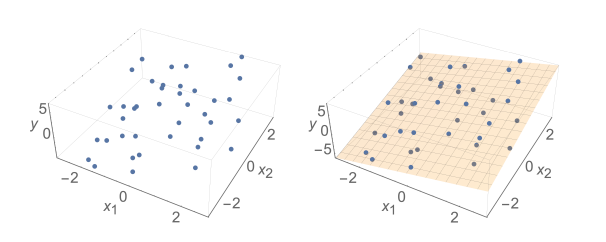
\includegraphics[width=100mm,scale=0.5]{images/regression_images/Regression_Plane.png}
        
            \caption*{This plane is \textbf{fitted} the same way our line was. Notice that $y$ is our \textbf{height}: this is the \textbf{output} of our regression.}
        \end{figure}
        
        Higher-dimension versions are hard to visualize. So, instead, we don't try, and call it a \textbf{hyperplane}.\\
        
        \begin{definition}
            A \vocab{hyperplane} is a \purp{higher-dimensional version} of a \gren{plane} - a \gren{flat} surface that continues on forever.
            
            We use it to represent our \gren{linear} hypothesis for the purpose of \purp{regression}. 
            
            The "\purp{height}" ($\nth{(d+1)}$ dimension) of this \gren{plane} at a certain point represents the \purp{output} of our \gren{linear} hypothesis at that point.
        \end{definition}
        
        Our line was a \textbf{1-D} object in a \textbf{2-D} plane. Our plane was a \textbf{2-D} object in a \textbf{3-D} space. So, our hyperplane is a $d$ dimensional object in a $d+1$ dimensional space.
        
        With this intuition, we can imagine our \textbf{hyperplane} as trying to get as \textbf{close} to all of the data points as it possibly can.
        
    \subsection*{Another Interpretation}
    
        There's another, similar way to interpret our model
        
        \begin{equation}
            h(x) = \red{\theta_0} + \red{\theta_1}x_1 + \red{\theta_2}x_2 + \red{\theta_3}x_3 + ... + \red{\theta_d}x_d
        \end{equation}
        
        Before, we took $\theta_k$ as just an \textbf{extension} of the $mx+b$ formula: $\theta_k$ tells us how much $x_k$ affects our output.
        
        However, we can also think about the \textbf{relative} scale of each $\theta_k$: if $\theta_2$ is \textbf{larger} than $\theta_1$, then $x_2$ has a \textbf{stronger} effect on the output than $x_1$.
        
        We can say that $x_2$ \textbf{weighs} more heavily in our calculation: it has more say in the \textbf{result}.
        
        Because of that, we sometimes call $\theta_k$ the \textbf{weight} for $x_k$.\\
        
        \begin{definition}
            A \vocab{weight} is a \gren{parameter} that tells us how \gren{strongly} a variable \purp{influences} our \purp{output}.
            
            It is usually a \purp{scalar} that we \gren{multiply} by our variable.
        \end{definition}
